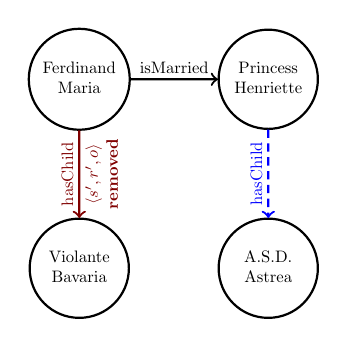
\begin{tikzpicture}[scale=0.6, every node/.style={scale=0.6}]
\node[draw,circle,thick,inner sep=0,minimum size=2.1cm] (r_fm) at (12,-5) {\begin{tabular}{c} Ferdinand \\ Maria \end{tabular}};
\node[draw,circle,thick,inner sep=0,minimum size=2.1cm] (r_ph) at (16,-5) {\begin{tabular}{c} Princess\\ Henriette\end{tabular}};
\node[draw,circle,thick,inner sep=0,minimum size=2.1cm] (r_vb) at (12,-9) {\begin{tabular}{c} Violante\\ Bavaria\end{tabular}};
\node[draw,circle,thick,inner sep=0,minimum size=2.1cm] (r_ny) at (16,-9) {\begin{tabular}{c} A.S.D.\\Astrea\end{tabular}};
\draw[->,thick] (r_fm) -- (r_ph) node[pos=0.5, sloped,align=center, above]{isMarried};
\draw[->,thick,red!50!black] (r_fm) -- (r_vb) node[pos=0.5, sloped,align=center, above]{hasChild} node[pos=0.5, sloped,align=center, below]{$\langle s',r',o\rangle$\\\textbf{removed}};
\draw[->,thick,blue,densely dashed] (r_ph) -- (r_ny) node[pos=0.5, sloped,align=center, above] {hasChild};
\end{tikzpicture}